Ce texte présente une équation aux dérivées partielles dont la résolution peut être vue comme une généralisation du calcul numérique d'une primitive. Il montre les problèmes de convergence attachés au choix d'un schéma particulier de discrétisation des dérivées. L'équation considérée est
\begin{equation}
 \frac{\partial u}{\partial t} + \frac{\partial u}{\partial x} = 0 \label{EqTransport}
\end{equation}
où $u$ est une fonction définie dans une partie $A$ de $\R^2$. La première composante d'un couple $(t,x)\in A$ représente un instant et la deuxième un point.\newline
Pour un point fixé représenté par $x$, notons 
\begin{itemize}
 \item $u_x$ la fonction définie dans une partie $I_x$ (intervalle de temps) de $\R$ qui à un instant $t$ associe $u((t,x))$,  
 \item $u_t$ la fonction définie dans une partie $J_t$ (intervalle d'espace) de $\R$ qui à un point $x$ associe $u((t,x))$,  
 \item $f$ la fonction définie dans $I_x$ qui à un instant $t$ associe $\frac{\partial u}{\partial x}((t,x))$.
\end{itemize}
On ajoute une \og condition aux limites\fg~ imposant, pour un instant fixé $t_0$ que $u_{t_0}$ est une fonction $v_0$ donnée à l'avance. L'équation s'écrit alors
\[
 u_x'(t) = -f(t) \hspace{1cm} u_x(t_0) = v(x).
\]
Pour chaque $x$, il s'agit donc bien d'un calcul de primitive d'une fonction de $t$. On admet que l'équation \ref{EqTransport} avec une condition aux limites $v$ admet une unique solution.\newline
Pour résoudre numériquement cette équation, on discrétise le temps et l'espace
\begin{itemize}
 \item $t_0, t_1, t_2, \cdots $: pas constant $t_{k+1} - t_k = \delta_t$ pour $k\in \llbracket 0, n_t \rrbracket$,
 \item $x_0, x_1, x_2, \cdots$:  pas constant $x_{l+1} - x_l = \delta_x$ pour $l\in \llbracket 0, n_x \rrbracket$
\end{itemize}
et on note $u_{k,l}$ au lieu de $u(t_k,x_l)$ et $v_l = v(x_l)$ pour $l\in \llbracket 0, n_x\rrbracket$ (fonction de la condition aux limites). On remplace alors la dérivée par un schéma numérique.\newline
Pour la dérivée par rapport au temps, on utilise
\[
 \frac{\partial u}{\partial t}(t_k,x_l) \simeq \frac{u(t_{k+1},x_l) - u(t_{k},x_l)}{\delta_t} = \frac{u_{k+1,l} - u_{k,l}}{\delta_t}.
\]
Pour la dérivée par rapport à l'espace, on envisage plusieurs schémas numériques dans le tableau suivant
\begin{center}
\renewcommand{\arraystretch}{2.4}
\begin{tabular}{|c|c|c|c|}\hline
schémas                                         & décentré à droite                                    & centré                                                  & décentré à gauche\\ \hline
$\dfrac{\partial u}{\partial x}(t_k,x_l) \simeq$ & $\dfrac{u_{k,l+1} - u_{k,l}}{\delta_x}$ & $\dfrac{u_{k,l+1} - u_{k,l-1}}{2\delta_x}$ & $\dfrac{u_{k,l} - u_{k,l-1}}{\delta_x}$ \\  \hline
\end{tabular}
\end{center}
Dans toute la suite, on suppose que pour tous les instants $t$, la fonction $u_t$ est périodique de période $1$. c'est donc le cas en particulier pour la fonction $v$ de la condition aux limites.
\begin{figure}[h]
 \centering
 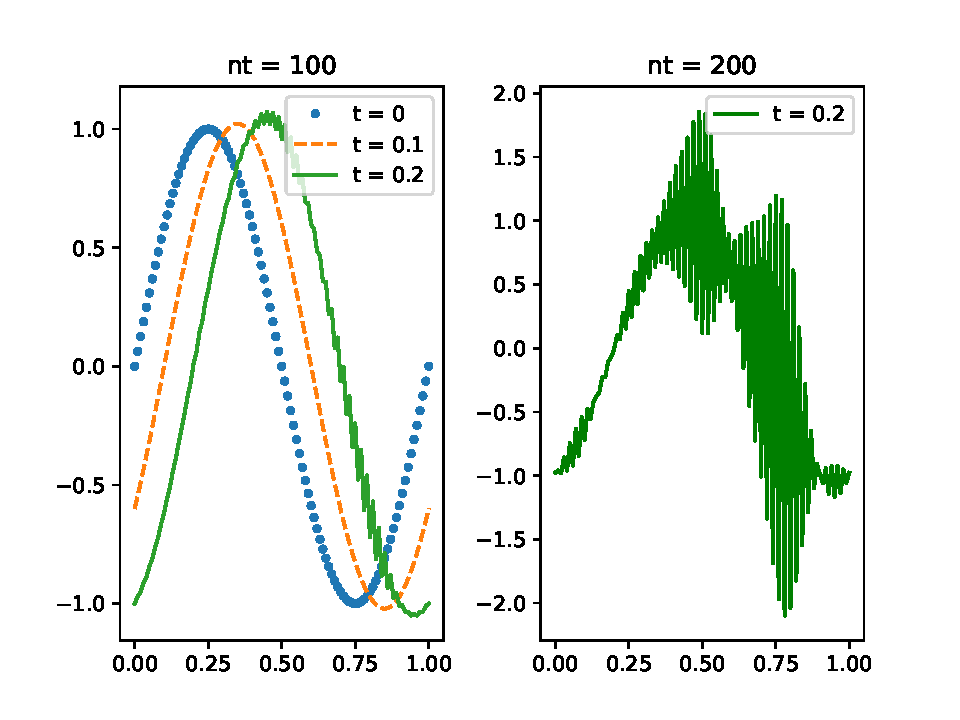
\includegraphics[width=10cm]{./Eequtransp_1.pdf}
 \caption{Schéma décentré à droite}
 \label{fig: Eequtransp_1}
\end{figure}

\begin{figure}[h]
 \centering
 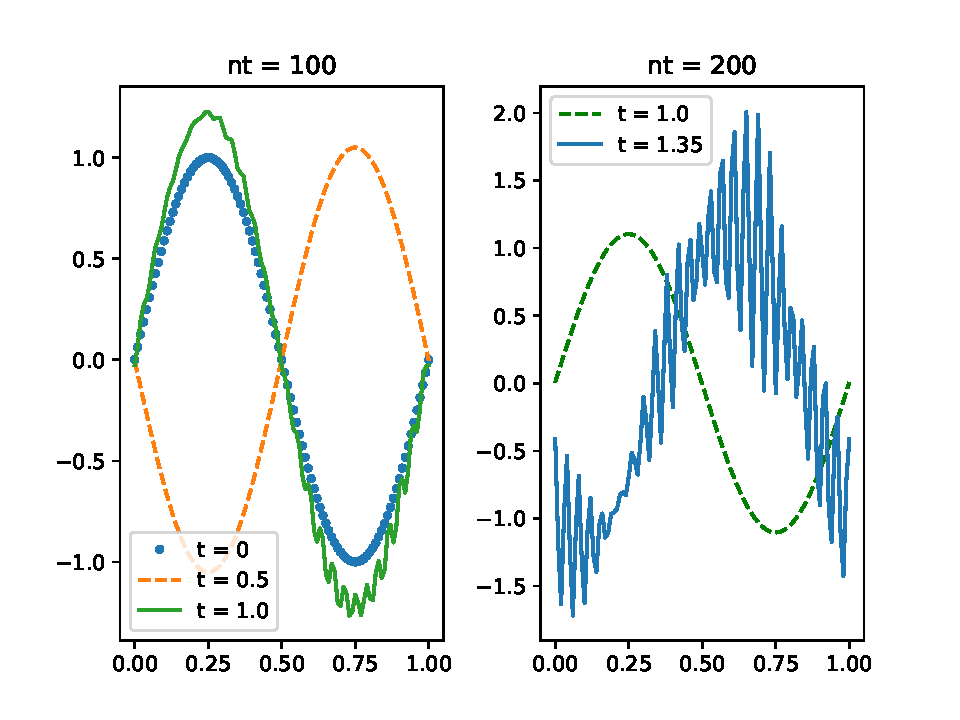
\includegraphics[width=10cm]{./Eequtransp_2.pdf}
 \caption{Schéma centré}
 \label{fig: Eequtransp_2}
\end{figure}

\begin{figure}[h]
 \centering
 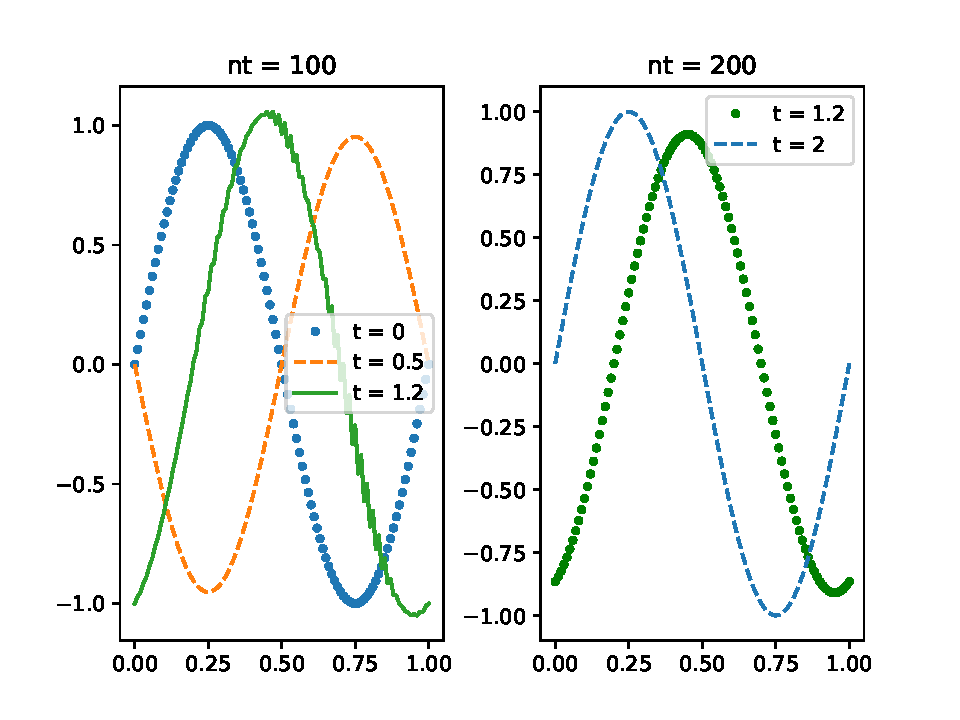
\includegraphics[width=10cm]{./Eequtransp_3.pdf}
 \caption{Schéma décentré à gauche}
 \label{fig: Eequtransp_3}
\end{figure}

\begin{enumerate}
 \item Pour chacun des trois schémas, former les relations permettant de calculer les $u_{k,l}$ avec $k\in \llbracket 0, n_t \rrbracket$ et $l\in \llbracket 0, n_x \rrbracket$.
 \item Pour un temps $t>0$, on veut évaluer numériquement la fonction $u_t$ d'une variable d'espace (on sait qu'elle est périodique de période $1$). On discrétise l'intervalle d'espace $[0,1]$ avec un pas $\delta_x = \frac{1}{n_x}$ pour $n_x$ entier et l'intervalle de temps $[0,t]$ avec un pas $\delta_t = \frac{t}{n_t}$ pour $n_t$ entier.\newline
 La condition initiale $v$ est donnée par une liste de $n_x$ valeurs $[v_0,v_1,\cdots ]$.
 \begin{enumerate}
  \item Former une fonction Python \texttt{transportDrte(t,nt,nx,v)} qui prend pour paramètres 
  \begin{itemize}
    \item un flottant \texttt{t} représentant un instant,
    \item des entiers \texttt{nt} et \texttt{nx} permettant de définir les pas en temps et en espace,
    \item une fonction \texttt{v} représentant la condition aux limites.
  \end{itemize}
Elle renvoie la liste des \texttt{nx}$+1$ flottants représentants les valeurs de la fonction $u_t$ aux points discrétisés calculés avec le schéma décentré à droite.

  \item Former une fonction Python \texttt{transportCtre(t,nt,nx,v)} analogue à la précédente mais pour le schéma centré.
  
  \item Former une fonction Python \texttt{transportGche(t,nt,nx,v)} analogue à la précédente mais pour le schéma décentré à gauche.
 \end{enumerate}
 
\item Pour évaluer la pertinence des méthodes proposées, on se place dans un cas pour lequel on connait l'expression d'une solution. Notons $S$ l'application définie dans $\R$ par:
\[
 \forall w\in \R, \; S(w) = \sin(2\pi\,w).
\]
\begin{enumerate}
 \item Montrer que la fonction $u$ définie dans $\R^2$ par:
\[
 \forall (t,x)\in \R^2, \; u((t,x)) = \sin(2\pi(x - t))
\]
est une solution de \ref{EqTransport} avec la condition aux limites $v = S$ pour $t_0=0$.
 \item Les figures \ref{fig: Eequtransp_1}, \ref{fig: Eequtransp_2}, \ref{fig: Eequtransp_3} présentent les graphes des évaluations des fonctions $u_t$ pour les trois schémas et diverses valeurs de $t$ et de $n_t$ (le nombre $n_x$ de points discrétisant l'espace est toujours $100$).\newline
 En examinant ces figures, que pouvez vous dire de la convergence des schémas lorsque le pas de temps $\delta_t = \frac{t}{n_t}$ devient petit?
\end{enumerate}

\item On revient aux notations de la question 1 et on suppose $\delta_t < \delta_x$. On pose
\[
 \forall k \in \llbracket 0, n_t\rrbracket, \; M_k = \max_{l \in \llbracket 0, n_x\rrbracket} \left| u_{k,l}\right|.
\]
Montrer les majorations suivantes pour les trois schémas
\begin{center}
\renewcommand{\arraystretch}{2.}
\begin{tabular}{|c|c|c|c|} \hline
Schéma        & décentré droite & centré & décentré gauche\\ \hline
$M_{k+1}\leq$ & $\left( 1+2\dfrac{\delta_t}{\delta_x}\right)M_k$  & $\left( 1 + \dfrac{\delta_t}{\delta_x}\right)M_k$ & $M_k$ \\ \hline
\end{tabular}
\end{center}

\end{enumerate}

